\documentclass[10pt,twocolumn,letterpaper]{article}

% =========================
% Packages
% =========================
\usepackage[margin=0.75in]{geometry}
\usepackage{amsmath, amssymb, amsthm}
\usepackage{mathtools}
\usepackage{microtype}
\usepackage{graphicx}
\graphicspath{{figures/}{../figures/}}
\usepackage{subcaption}
\usepackage{booktabs}
\usepackage{multirow}
\usepackage{array}
\usepackage{tabularx}
\usepackage[hypertexnames=false]{hyperref}
\usepackage{url}
\usepackage{algorithm}
\usepackage{algpseudocode}
\usepackage{enumitem}

% =========================
% Theorem Environments
% =========================
\newtheorem{theorem}{Theorem}
\newtheorem{lemma}{Lemma}
\newtheorem{proposition}{Proposition}
\newtheorem{corollary}{Corollary}
\theoremstyle{definition}
\newtheorem{definition}{Definition}
\newtheorem{assumption}{Assumption}
\newtheorem{remark}{Remark}

% =========================
% Commands
% =========================
\newcommand{\R}{\mathbb{R}}
\newcommand{\stiefel}{\mathrm{St}}
\newcommand{\Sigmahat}{\widehat{\Sigma}}
\DeclareMathOperator{\prox}{prox}
\DeclareMathOperator{\soft}{soft}
\DeclareMathOperator{\supp}{supp}
\DeclareMathOperator{\tr}{tr}
\DeclareMathOperator{\sym}{sym}
\DeclareMathOperator{\dist}{dist}
\newcolumntype{Y}{>{\raggedright\arraybackslash}X}
\setlength{\columnsep}{0.25in}
\setlength{\emergencystretch}{3em}
\hbadness=10000
\graphicspath{{figures/}{../figures/}}

% =========================
% Title
% =========================
\title{\texorpdfstring{When Graph Regularization Helps (and Hurts): Topology-Dependent Regimes in Sparse PCA}{When Graph Regularization Helps (and Hurts): Topology-Dependent Regimes in Sparse PCA}}
\author{Wang Zhoufu}
\date{}

\begin{document}
\sloppy
\raggedbottom
\maketitle

% =========================
% Abstract
% =========================
\begin{abstract}
We study sparse, graph-smooth, explicitly orthogonal multi-component PCA through a split-variable formulation that couples an orthogonal loading matrix with a sparse graph-regularized proxy. We propose a concrete alternating solver consisting of a Stiefel manifold update for the orthogonal factor and a proximal-gradient update for the sparse graph-smooth factor. We evaluate the method on synthetic chain and grid graphs under controlled graph misspecification, reporting support recovery, graph smoothness on the true graph, and shared explained variance. The results support a regime-based view: at low $\lambda_2$ the method is robust to misspecification across topologies, while at higher $\lambda_2$ misspecification effects depend on topology, with fragile chain graphs degrading under rewiring and redundant grid graphs remaining largely invariant. Empirically, moderate $\lambda_2$ yields favorable variance--smoothness tradeoffs before stronger regularization leads to diminishing returns. We therefore position our contribution as a regime-level characterization of when graph regularization is reliable under misspecification, rather than as an across-the-board performance improvement.
\end{abstract}

\section{Introduction}
\label{sec:introduction}

Principal component analysis (PCA) is a foundational technique for dimensionality reduction, exploratory analysis, and low-dimensional representation learning. Its appeal stems from its simplicity and its optimality for variance maximization under orthogonality constraints. However, classical PCA typically produces dense loading vectors, so that each principal component depends on nearly all input variables. In modern high-dimensional applications such as genomics, neuroimaging, and structured sensing, these dense loadings can be difficult to interpret and of limited use for scientific discovery or feature selection \cite{zou2006spca,chen2020amanpg}.

Sparse principal component analysis (SPCA) addresses this limitation by encouraging principal components to depend on only a small subset of variables. Over the past two decades, SPCA has been studied through several complementary formulations, including regression-based relaxations, power-method variants, and nonsmooth constrained optimization approaches \cite{zou2006spca,journee2010gpower,chen2020amanpg}. More recent work has emphasized the importance of handling sparsity and orthogonality in a principled manner, rather than relying solely on heuristic thresholding or post hoc orthogonalization. In particular, manifold-based formulations such as alternating manifold proximal-gradient methods show that sparse multi-component estimation can be treated directly as a nonsmooth optimization problem with orthogonality constraints, yielding stronger algorithmic structure and convergence guarantees than purely heuristic alternatives \cite{chen2020amanpg,chen2024nonsmoothstiefel}.

Despite these advances, sparsity alone is often not enough. In many high-dimensional domains, features are not exchangeable but are linked through known relational structure. Genes participate in pathways and interaction networks, voxels exhibit spatial or functional connectivity, and pixels or spectral bands obey spatial adjacency and smoothness patterns. When such prior structure is available, it is natural to ask whether the extracted principal components should also respect it. A large literature on graph-aware and graph-regularized PCA studies how incorporating structural priors through graph-based penalties or low-frequency graph constraints can improve robustness and structural fidelity, especially when the signal is aligned with the underlying graph \cite{briola2026grpca}. At the same time, this literature also makes clear that graph-aware PCA is not a single unified model class: some methods emphasize low-frequency graph consistency, some include explicit sparsification, and others target application-specific clustering or representation objectives rather than sparse orthogonal component extraction \cite{briola2026grpca,feng2019glspca,wu2019gdspca,wang2025rsspca}.

A second challenge concerns the extraction of multiple components. In classical PCA, orthogonality follows directly from eigendecomposition. In sparse settings, however, orthogonality is no longer automatic, and sequential deflation can produce components that are only approximately orthogonal or that degrade cumulatively in quality. This has motivated a continued line of work on simultaneous sparse orthogonal extraction, including recent efforts that explicitly revisit orthogonal SPCA as an active optimization problem rather than a solved issue \cite{chen2020amanpg,bertsimas2023geospca,cheng2026orthogonalspca}. These developments suggest that, when multiple interpretable components are required, joint extraction under explicit orthogonality constraints remains preferable to treating sparsity as a purely post-processing step.

There is also a broader methodological backdrop. Beyond SPCA itself, recent work on nonsmooth and structured nonsmooth optimization over Riemannian submanifolds has substantially expanded the toolkit available for nonconvex problems with manifold constraints \cite{li2024structurednonsmooth,chen2024nonsmoothstiefel}. Moreover, adjacent problems such as sparse tensor canonical correlation analysis already combine Laplacian regularization, sparse penalties, manifold-based optimization, and modern inner solvers with convergence analysis \cite{zhu2025stccal}. Consequently, it is no longer accurate to position graph-coupled nonsmooth manifold optimization as an entirely unexplored conceptual territory. Rather, the more defensible and practically meaningful question is whether these ideas can be brought together in a coherent and effective framework for \emph{PCA proper}, with an explicit focus on sparse multi-component loading estimation under feature-graph smoothness and simultaneous orthogonality.

This paper studies that question. We consider a formulation that combines three desiderata: sparse loadings, smoothness with respect to a known feature graph, and joint orthogonality across multiple extracted components. Our goal is not to claim that graph-aware PCA, graph+sparsity PCA, or nonsmooth manifold optimization are individually new. Instead, we focus on a comparatively underexplored intersection of these themes: \emph{feature-graph Laplacian regularization, sparse multi-component loadings, and explicit simultaneous orthogonality within a modern manifold/proximal optimization framework for PCA}. This positioning is narrower than a broad novelty claim, but it better reflects the current state of the literature and the genuine methodological gap that remains \cite{briola2026grpca,feng2019glspca,wu2019gdspca,chen2020amanpg}.

Concretely, we introduce a graph-smooth sparse orthogonal PCA formulation in which orthogonality is handled through a Stiefel-constrained variable and structured sparse estimation is handled through a graph-regularized Euclidean variable coupled by a quadratic penalty. This split allows us to separate the geometry of orthogonality from the graph-coupled sparsity structure, while still optimizing the two jointly. The resulting viewpoint is particularly attractive in settings where interpretability is not just a matter of selecting a few variables, but of selecting variables whose pattern is coherent with known domain structure.

Our study is guided by two central questions. First, when does feature-graph regularization preserve recovery while improving structural coherence of sparse components? Second, what tradeoff does graph regularization induce between explained variance, graph consistency, and computational cost? These questions are important because graph-based regularization can help when the prior graph is informative, but may oversmooth the loadings or reduce variance capture when the graph is misspecified. Accordingly, the paper emphasizes not only model design and optimization, but also the empirical circumstances under which graph priors are beneficial, revealing a phase diagram over regularization strength and corruption level.

\paragraph{Contributions.}
The main contributions of this work are as follows.
\begin{itemize}[leftmargin=*]
    \item We study graph-regularized sparse orthogonal PCA under controlled misspecification and show that the effect of graph regularization is regime-dependent in $\lambda_2$.
    \item On chain graphs, stronger regularization amplifies misspecification effects, with rewiring more harmful than edge deletion; on grid graphs, performance is near-invariant under the same perturbations, indicating that robustness to misspecification is topology-dependent.
    \item We identify an \emph{illusory smoothness} phenomenon, where graph misspecification can yield smoother solutions under the imposed prior without improving alignment with the true graph.
    \item We provide a concrete split-variable solver that combines explicit orthogonality, sparsity, and graph smoothness within a single executable framework.
\end{itemize}

Taken together, these contributions position the paper as a targeted integration of ideas that already exist in neighboring literatures, but whose precise combination for graph-smooth sparse orthogonal PCA remains comparatively underdeveloped. Our aim is therefore not to argue that every ingredient is new, but to show that their combination leads to a useful and well-motivated framework for structured dimensionality reduction in graph-informed high-dimensional settings.

\section{Related Work}
\label{sec:related}

\subsection{Sparse PCA and Orthogonal Component Extraction}
Sparse principal component analysis has been studied through regression-based relaxations, truncated power methods, penalized matrix decomposition, semidefinite relaxations, and nonsmooth constrained optimization \cite{zou2006spca,witten2009pmd,daspremont2007dspca,journee2010gpower,qiu2023gradientspca}. A central theme in this literature is that sparse loadings improve interpretability but complicate both optimization and the extraction of multiple components.

A particularly important line of work formulates SPCA directly as a nonsmooth optimization problem over orthogonality-constrained variables. Chen et al.\ proposed the alternating manifold proximal gradient framework (A-ManPG) for sparse PCA and sparse CCA, showing that sparse loadings and nonconvex orthogonality constraints can be handled within a unified manifold-based optimization scheme with convergence guarantees \cite{chen2020amanpg}. More broadly, the ManPG literature establishes a practical optimization template for smooth-plus-nonsmooth objectives on the Stiefel manifold \cite{chen2020manpg,chen2024nonsmoothstiefel}.

Orthogonal sparse extraction also remains an active topic rather than a closed one. GeoSPCA emphasizes simultaneous extraction over deflation for orthogonal sparse components \cite{bertsimas2023geospca}, and recent work on certifiably optimal orthogonal SPCA further underscores ongoing interest in jointly enforcing sparsity, orthogonality, and strong optimality properties \cite{cheng2026orthogonalspca}. These developments motivate explicit joint orthogonality rather than treating it as an afterthought.

\subsection{Graph-Aware PCA and Graph-Regularized Dimensionality Reduction}
A parallel literature incorporates structural priors into PCA through graphs or Laplacian-type regularization. These methods are motivated by the observation that in many high-dimensional applications, features are not exchangeable but related through biological, spatial, or network structure. Graph-aware PCA methods use this prior information to bias principal components toward graph-consistent directions, often by suppressing high-frequency variation and preserving graph-coherent low-frequency signals \cite{briola2026grpca,chung1997spectral,shuman2013gsp}.

Recent work makes it clear that graph-regularized PCA cannot simply be characterized as producing dense loadings. In particular, GR-PCA incorporates a learned sparse precision graph and regularizes PCA toward the low-frequency Fourier modes of the induced graph Laplacian; the method also evaluates sparsity-related behavior explicitly and reports improved structural fidelity, lower Laplacian energy, and competitive out-of-sample reconstruction under graph-aligned signals \cite{briola2026grpca}. This weakens any broad claim that graph-aware PCA is predominantly dense or uninterpretable.

At the same time, graph-aware PCA does not fully eliminate the gap relevant here. Many graph-regularized variants focus primarily on graph consistency, robustness, clustering structure, or low-frequency filtering, rather than on simultaneous sparse multi-component orthogonality in a single PCA-specific framework. Accordingly, the relevant distinction is no longer whether graph-aware PCA exists, but whether it addresses the specific combination of sparse loadings, feature-graph smoothness, and explicit joint orthogonality considered here.

\subsection{Graph + Sparsity PCA Variants}
Older and application-driven papers already show that graph structure and sparsity have been combined within PCA-like models. For example, gLSPCA integrates a graph Laplacian term and a sparsity constraint into PCA for gene-expression analysis \cite{feng2019glspca}, while GDSPCA combines graph Laplacian regularization with double sparsity constraints to improve interpretability and exploit internal geometry \cite{wu2019gdspca}. These papers are direct counterexamples to any claim that graph+sparsity PCA is absent from the literature.

However, these graph+sparsity PCA methods also illustrate why the gap must be phrased carefully. They are often application-specific, may target particular geometric or clustering objectives, and do not necessarily adopt the same optimization language as modern manifold proximal methods for joint orthogonal extraction. Recent applied work such as RSSPCA reinforces the same point: smooth sparse PCA variants continue to emerge in domain-specific settings, but they do not by themselves close the gap for feature-graph Laplacian regularization with explicit simultaneous orthogonal extraction in PCA proper \cite{wang2025rsspca}.

\subsection{Structured Sparse PCA}
Structured sparse PCA extends plain $\ell_1$-based sparsity by encouraging supports that follow meaningful patterns such as groups, trees, or contiguous regions. Jenatton, Obozinski, and Bach showed that structured regularization can impose higher-order information on the support of loading vectors and can improve interpretability relative to unstructured sparse PCA \cite{jenatton2010sspca}. This literature is highly relevant because it demonstrates that sparsity alone is often too weak a prior.

Nevertheless, structured sparse PCA in this sense is not identical to feature-graph smoothness. Structured sparsity typically constrains the support geometry through groups or shapes, whereas graph-Laplacian regularization encourages neighboring or strongly connected features to take similar values. These are related but distinct inductive biases, and the existence of structured sparse PCA does not by itself resolve the specific question of how to jointly impose graph smoothness, sparsity, and simultaneous orthogonality in multi-component PCA.

\subsection{Structured Nonsmooth Optimization on Manifolds}
The optimization backdrop for this problem has evolved substantially. Beyond the sparse-PCA-specific literature, recent work on nonsmooth and structured nonsmooth optimization over Riemannian submanifolds shows that manifold-based methods now handle a broader class of composite objectives than earlier sparse-only formulations \cite{li2024structurednonsmooth,chen2024nonsmoothstiefel}. Recent adjacent work also combines sparse regularization, Laplacian regularization, manifold proximal updates, semismooth Newton subproblem solvers, and convergence analysis in related problems such as sparse tensor CCA \cite{zhu2025stccal}. That literature does not solve our PCA formulation directly, but it does weaken any broad claim that the optimization ingredients themselves are unprecedented.

\subsection{Positioning of the Present Work}
Graph-aware PCA and graph-regularized sparse PCA have been studied in multiple forms, and we do not claim novelty in combining graph smoothness with sparsity. The specific gap we target is the joint extraction of multiple explicitly orthogonal components under a split-variable formulation with a concrete, reproducible solver. Our work is positioned as a focused intersection of sparse PCA, graph-regularized PCA, and orthogonality-preserving optimization, rather than as a first instance of any single ingredient.

\section{Problem Setup}
\label{sec:setup}

Let $X \in \R^{n \times p}$ be a centered data matrix and let
\begin{equation}
    \Sigmahat = \frac{1}{n} X^\top X
\end{equation}
denote the sample covariance matrix. Let $G=(\mathcal{V},\mathcal{E},W)$ be a weighted undirected feature graph on the $p$ variables, with adjacency matrix $W$, degree matrix $D$, and graph Laplacian
\begin{equation}
    L = D - W.
\end{equation}
We assume $L \succeq 0$.
We use $\|M\|_1$ for the entrywise $\ell_1$ norm, $\soft(Z,\tau)$ for entrywise soft-thresholding at threshold $\tau$, and $\sym(M) = (M+M^\top)/2$ for the symmetric part of a matrix. Shared explained variance is computed after QR-based orthonormalization of the loading matrix.

Our goal is to extract $r$ principal components with loading structure that is simultaneously sparse, graph-smooth, and orthogonal. To separate the geometry of orthogonality from the structured regularization, we introduce two variables $A,B \in \R^{p \times r}$:
\begin{itemize}[leftmargin=*]
    \item $A$ carries the orthogonality constraint $A^\top A = I_r$,
    \item $B$ carries sparsity and graph smoothness.
\end{itemize}

We denote the Stiefel manifold by
\begin{equation}
    \stiefel(p,r) = \{ A \in \R^{p \times r} : A^\top A = I_r \}.
\end{equation}

\section{Proposed Formulation}
\label{sec:formulation}

We study the split formulation
\begin{equation}
\label{eq:main_obj}
\begin{aligned}
\min_{A \in \stiefel(p,r),\, B \in \R^{p \times r}} \quad
&-\tr(A^\top \Sigmahat A)
+ \lambda_1 \|B\|_1 \\
&+ \lambda_2 \tr(B^\top L B)
+ \frac{\rho}{2}\|A-B\|_F^2.
\end{aligned}
\end{equation}

The first term promotes variance capture; the $\ell_1$ term promotes sparse loadings; the Laplacian term promotes graph smoothness; and the quadratic coupling term forces the orthogonal variable $A$ and the structured loading variable $B$ to remain close.

\paragraph{Penalty coupling.}
The coupling term $\frac{\rho}{2}\|A-B\|_F^2$ is a fixed-$\rho$ quadratic penalty that enforces approximate consensus between $A$ and $B$; we do not use dual variables or ADMM-style updates.

\paragraph{Why split variables?}
Directly optimizing a sparse graph-regularized objective under orthogonality constraints is difficult because the orthogonality constraint is nonconvex while the graph-sparsity regularizer is nonsmooth and coupled across features. The split formulation isolates these effects: $A$ is updated on the Stiefel manifold, while $B$ is updated in Euclidean space under structured regularization.

We leave alternative sparsity structures to future work to keep the formulation fixed to entrywise $\ell_1$ on $B$.

\section{Optimization Algorithm}
\label{sec:algorithm}

We solve the split-variable objective by alternating between two steps. The $A$-step updates an orthogonal loading matrix on the Stiefel manifold using a Riemannian gradient step followed by QR-based retraction. The $B$-step updates the sparse graph-smooth proxy with proximal gradient, treating the Laplacian quadratic and coupling term as the smooth part and the $\ell_1$ penalty as the nonsmooth part. This single solver path provides a minimal, reproducible baseline for the empirical study; more advanced variants remain future work.

\subsection{A-Step: Manifold Update}
With $B$ fixed, the $A$-subproblem is
\begin{equation}
\label{eq:A_subproblem}
\min_{A \in \stiefel(p,r)}
-\tr(A^\top \Sigmahat A)
+ \frac{\rho}{2}\|A-B\|_F^2.
\end{equation}
Its Euclidean gradient is
\begin{equation}
    \nabla_A f(A;B) = -2\Sigmahat A + \rho (A-B).
\end{equation}
The corresponding Riemannian gradient on $\stiefel(p,r)$ is
\begin{equation}
    \operatorname{grad} f(A;B)
    = \nabla_A f(A;B) - A\,\sym\!\big(A^\top \nabla_A f(A;B)\big).
\end{equation}
We take a fixed-step manifold descent update with step size $\eta_A$ and retract back to the Stiefel manifold using QR retraction.

\subsection{B-Step: Graph-Coupled Sparse Update}
With $A$ fixed, the $B$-subproblem is
\begin{equation}
\label{eq:B_subproblem}
\min_{B \in \R^{p \times r}}
\lambda_1 \|B\|_1
+ \lambda_2 \tr(B^\top L B)
+ \frac{\rho}{2}\|A-B\|_F^2.
\end{equation}
This subproblem is convex in $B$ because $L \succeq 0$. We use a proximal-gradient update that treats the Laplacian quadratic and coupling term as the smooth part and the $\ell_1$ penalty as the nonsmooth part. Define
\[
g(B) = \lambda_2 \tr(B^\top L B) + \frac{\rho}{2}\|A-B\|_F^2,
 \qquad
h(B) = \lambda_1 \|B\|_1.
\]
Then
\[
\nabla g(B) = 2\lambda_2 L B + \rho(B-A).
\]
With step size $\eta_B = 1 / (2\lambda_2 \|L\|_2 + \rho)$, the update is
\[
B^{(t+1)} = \soft\!\big(B^{(t)} - \eta_B \nabla g(B^{(t)}), \eta_B \lambda_1\big).
\]

\subsection{Alternating Scheme}
Algorithm~\ref{alg:alt} summarizes the outer loop.

\begin{algorithm}[t]
\caption{Alternating Manifold + Graph-Coupled Sparse Updates}
\label{alg:alt}
\begin{algorithmic}[1]
\Require Centered data $X$, graph Laplacian $L$, parameters $\lambda_1,\lambda_2,\rho$, rank $r$
\State Initialize $A^{(0)} \in \stiefel(p,r)$, $B^{(0)} \in \R^{p\times r}$
\For{$t=0,1,\dots,T-1$}
\State Update $A^{(t+1)}$ with one Riemannian gradient step and QR retraction
\State Update $B^{(t+1)}$ with one proximal-gradient step and soft-thresholding
    \If{stopping criterion satisfied}
        \State \textbf{break}
    \EndIf
\EndFor
\State \Return $(A^{(T)},B^{(T)})$
\end{algorithmic}
\end{algorithm}

\paragraph{Complexity.}
The cost of the $A$-step is dominated by matrix multiplications and the chosen retraction. The $B$-step is typically the computational bottleneck because graph regularization introduces feature coupling and removes the closed-form separability available in plain soft-thresholding. When $L$ is sparse, matrix-vector operations remain efficient; dense or ill-conditioned graph operators can substantially increase runtime.

\section{Optimization Discussion}
\label{sec:theory}

The objective in \eqref{eq:main_obj} is nonconvex because it combines a Stiefel constraint on $A$ with a quadratic coupling term between $A$ and $B$. For fixed $A$, however, the $B$-subproblem is convex because it is the sum of a convex quadratic term and the entrywise $\ell_1$ norm.

\subsection{Updates Used}
The implemented solver alternates between two explicit updates. The $A$-step takes one retracted Riemannian gradient step on $\stiefel(p,r)$ using the Euclidean gradient from the manifold objective and QR retraction back to the manifold. The $B$-step takes one proximal-gradient step, with the smooth part given by the Laplacian quadratic and coupling term and the nonsmooth part given by $\lambda_1 \|B\|_1$.

The step size for the $A$-step is fixed at $\eta_A=0.05$. This value is conservative relative to the Lipschitz bound for the smooth $A$-subproblem (on the order of $2\|\Sigmahat\|_2 + \rho$), and was not tuned to optimize evaluation metrics. The $B$-step uses
\[
\eta_B = \frac{1}{2\lambda_2 \|L\|_2 + \rho},
\]
which matches the Lipschitz constant of the smooth part in the Euclidean update. We compute $\|L\|_2$ as the largest eigenvalue of $L$ (via \texttt{eigvalsh}).

\subsection{Stopping Criteria}
The outer loop stops when any of the following is satisfied (defaults used in all reported runs):
\begin{itemize}[leftmargin=*]
    \item relative objective change $\le 10^{-6}$,
    \item coupling gap $\|A-B\|_F / \max(1,\|A\|_F) \le 10^{-4}$,
    \item orthogonality defect $\|A^\top A - I_r\|_F \le 10^{-6}$,
    \item maximum iteration count $T=200$ is reached.
\end{itemize}

This section is intentionally descriptive rather than a proof development: we do not provide a formal convergence proof here, and formal analysis is out of scope for this manuscript.

\section{Experiments}
\label{sec:experiments}

\paragraph{Overview.}
We map when graph regularization helps versus hurts by varying regularization strength and topology under controlled misspecification. We focus on chain and grid graphs with a fixed $\lambda_2$ sweep to probe the low-to-moderate regime. The goal is regime characterization, not absolute performance gains.

\paragraph{Experimental setup.}
We evaluate chain and grid graph families only. Graph corruption is applied to the \emph{prior} graph used by the method; synthetic data and true supports are generated from the clean graph, so the study measures misspecification rather than altered ground truth. We consider two corruption types---edge deletion and random rewiring---with a fixed corruption level $\alpha=0.2$ (fraction of $|E|$). We sweep $\lambda_2 \in \{0, 0.01, 0.02, 0.05, 0.1, 0.2, 0.5, 1.0\}$ with seeds $\{0,1,2\}$ (3 seeds for consistency checks, not statistical claims). Metrics reported are support recovery (F1), graph smoothness on the true graph, and shared explained variance. Baselines include PCA, A-ManPG, SparseNoGraph ($\lambda_2=0$), and the Proposed method. All methods are implemented in NumPy.

\subsection{Effect of Regularization Strength (Chain)}
Figure~\ref{fig:phase2-chain} shows the $\lambda_2$ sweep on chain graphs under clean, delete, and rewire priors. At low $\lambda_2$, curves overlap, indicating robustness when the graph prior is weak. At higher $\lambda_2$, the chain becomes misspecification-sensitive: clean retains higher recovery, deletion degrades moderately, and rewire degrades most. This establishes the chain mechanism—strong regularization amplifies errors in local adjacency.

\subsection{Topology-Dependent Robustness (Chain vs Grid)}
Figure~\ref{fig:phase2-compare} contrasts chain and grid under the same corruption and $\lambda_2$ sweep. The chain exhibits clear degradation under rewiring at moderate-to-high $\lambda_2$, while grid graphs remain largely invariant under the same perturbations. Quantitatively, the clean--rewire gap in support F1 at $\lambda_2=0.5$ and $1.0$ is $+0.058$ and $+0.076$ for the chain, but $-0.041$ and $-0.028$ for the grid. The small sign changes on the grid indicate that misspecification effects are weak and unstable in direction, consistent with robustness rather than genuine benefit.

\subsection{Signal--Graph Compatibility}
We vary support structure to isolate when the graph prior matches the signal. Figure~\ref{fig:compat-chain} and Figure~\ref{fig:compat-grid} show that graph-aligned supports (connected or multi-cluster) achieve higher recovery than fragmented supports across the $\lambda_2$ sweep. On SBM (Figure~\ref{fig:compat-sbm}), cross-community supports degrade more rapidly at moderate-to-high $\lambda_2$ than within-community supports, indicating that mismatch between signal structure and graph topology amplifies the cost of strong regularization.

\subsection{Multi-Component Validation}
We test whether the observed regimes persist when extracting multiple components on SBM graphs. Figure~\ref{fig:multicomp-connected}, Figure~\ref{fig:multicomp-fragmented}, and Figure~\ref{fig:multicomp-cross} summarize mean per-component recovery and orthogonality error for $r \in \{2,3,5\}$. Across SBM regimes (connected, fragmented, and cross-community), a consistent regime pattern emerges: low--to--moderate $\lambda_2$ yields stronger recovery, while higher $\lambda_2$ leads to substantial degradation. Orthogonality remains stable across all settings, indicating that the observed degradation arises from over-regularization rather than optimization instability.

\subsection{Corruption-Strength Sweep (Chain)}
Figure~\ref{fig:phase2-alpha} reports a phase diagram over $(\lambda_2, \alpha)$ for chain graphs, with separate panels for deletion and rewiring. Misspecification effects strengthen with increasing $\alpha$, and the most pronounced degradation occurs when both $\lambda_2$ and $\alpha$ are large. The diagram summarizes the regime boundary between robust low-$\lambda_2$ behavior and high-$\lambda_2$ sensitivity to corruption.
As $\alpha$ increases, the low-$\lambda_2$ region remains relatively stable, while high-$\lambda_2$ performance degrades more sharply, indicating that corruption strength and regularization jointly determine the regime boundary.

\subsection{Real-Data Sanity Check (TCGA-BRCA + STRING)}
We run a $\lambda_2$ sweep on TCGA-BRCA expression with a STRING PPI graph using three random initializations and report smoothness and shared explained variance (Figure~\ref{fig:realdata}). We observe that moderate $\lambda_2$ yields stable variance--smoothness tradeoffs, while larger $\lambda_2$ leads to more aggressive smoothing with diminishing variance gains, consistent with the synthetic regime behavior. A subsampling robustness sweep (Figure~\ref{fig:realdata-robust}) shows the same qualitative pattern across random subsamples.

\subsection{Interpretation}
The $\lambda_2$ axis controls prior strength, moving from weak to strong regularization. The topology axis distinguishes fragile graphs (chains) from redundant graphs (grids). The experiments show that misspecification sensitivity depends jointly on regularization strength and topology: strong graph regularization amplifies misspecification on fragile structures, while redundant topologies yield near-invariant performance. We also observe illusory smoothness: rewiring can increase smoothness measured under the corrupted prior without improving alignment with the true graph, particularly when recovery degrades.

\begin{figure}[t]
\centering
\includegraphics[width=\linewidth]{phase2/blockA/blockA_sanity_lambda2_sweep.png}
\caption{$\lambda_2$ sweep on chain graphs under clean, delete, and rewire priors. At low $\lambda_2$, all conditions behave similarly; at higher $\lambda_2$, misspecification induces clear degradation, with rewiring most harmful.}
\label{fig:phase2-chain}
\end{figure}

\begin{figure}[t]
\centering
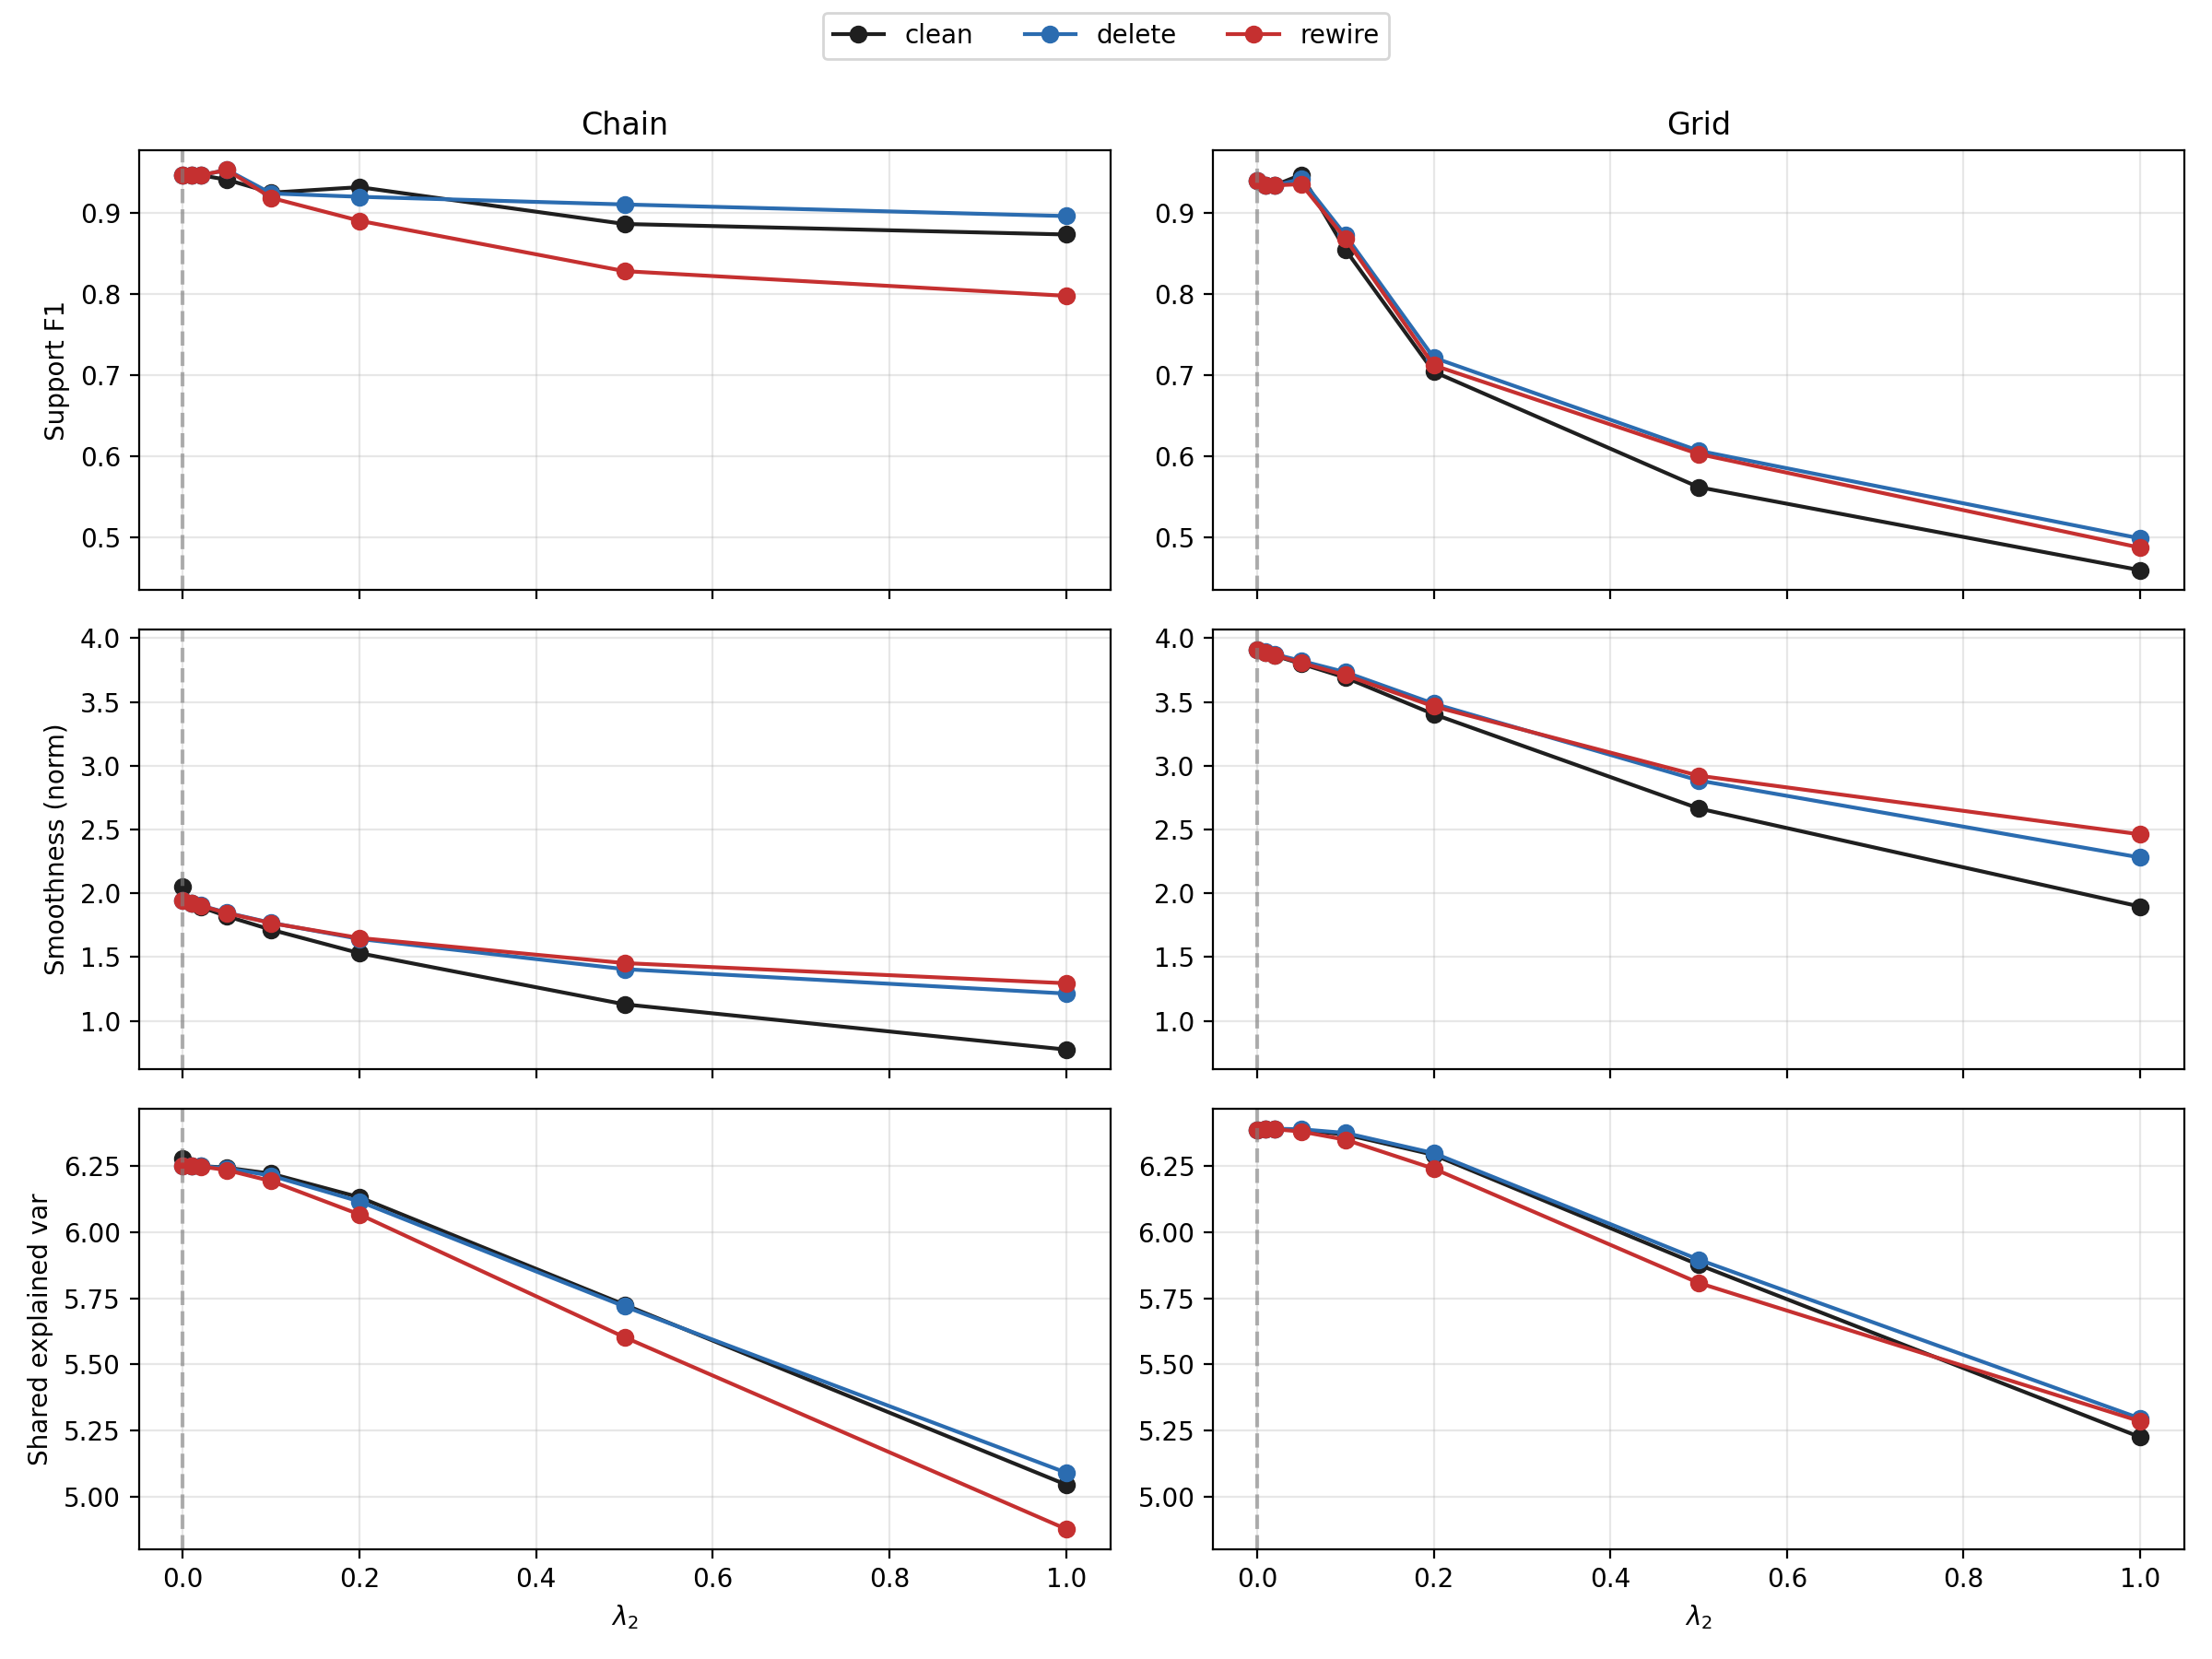
\includegraphics[width=\linewidth]{phase2/compare/blockAB_chain_grid_lambda2_sweep.png}
\caption{Effect of graph misspecification across graph topologies. Chain graphs (left) show increasing degradation under misspecification as $\lambda_2$ grows, with rewiring more harmful than edge deletion. Grid graphs (right) remain largely invariant under the same perturbations, indicating that misspecification sensitivity depends jointly on regularization strength and topology.}
\label{fig:phase2-compare}
\end{figure}

\begin{figure}[t]
\centering
\includegraphics[width=\linewidth]{phase2/compatibility/compat_chain_lambda2_sweep.png}
\caption{Compatibility sweep on chain graphs. Graph-aligned supports (connected, multi-cluster) maintain higher recovery than fragmented supports as $\lambda_2$ increases.}
\label{fig:compat-chain}
\end{figure}

\begin{figure}[t]
\centering
\includegraphics[width=\linewidth]{phase2/compatibility/compat_grid_lambda2_sweep.png}
\caption{Compatibility sweep on grid graphs. Recovery is highest for connected and multi-cluster supports and declines more sharply for fragmented supports at larger $\lambda_2$.}
\label{fig:compat-grid}
\end{figure}

\begin{figure}[t]
\centering
\includegraphics[width=\linewidth]{phase2/compatibility/compat_sbm_lambda2_sweep.png}
\caption{Compatibility sweep on SBM graphs. Cross-community supports degrade more rapidly at moderate-to-high $\lambda_2$ than within-community supports, indicating a mismatch penalty.}
\label{fig:compat-sbm}
\end{figure}

\begin{figure}[t]
\centering
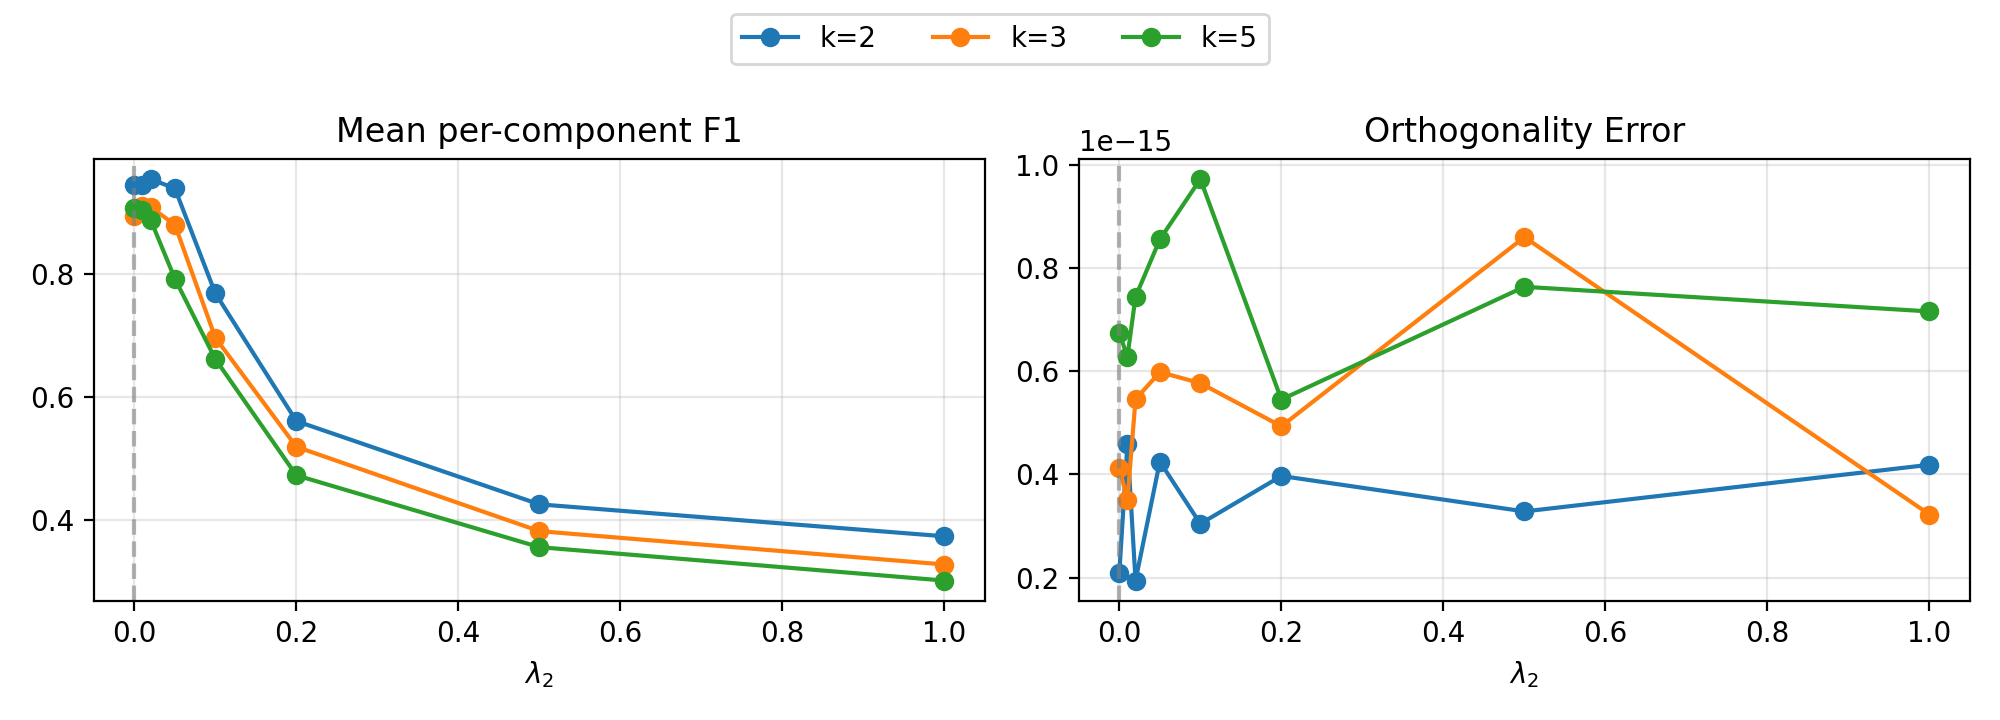
\includegraphics[width=\linewidth]{phase2/multicomponent/multicomp_connected_lambda2_sweep.png}
\caption{Multi-component sweep on SBM graphs with connected supports. Mean per-component F1 and orthogonality error remain stable at low-to-moderate $\lambda_2$ and degrade only at higher regularization.}
\label{fig:multicomp-connected}
\end{figure}

\begin{figure}[t]
\centering
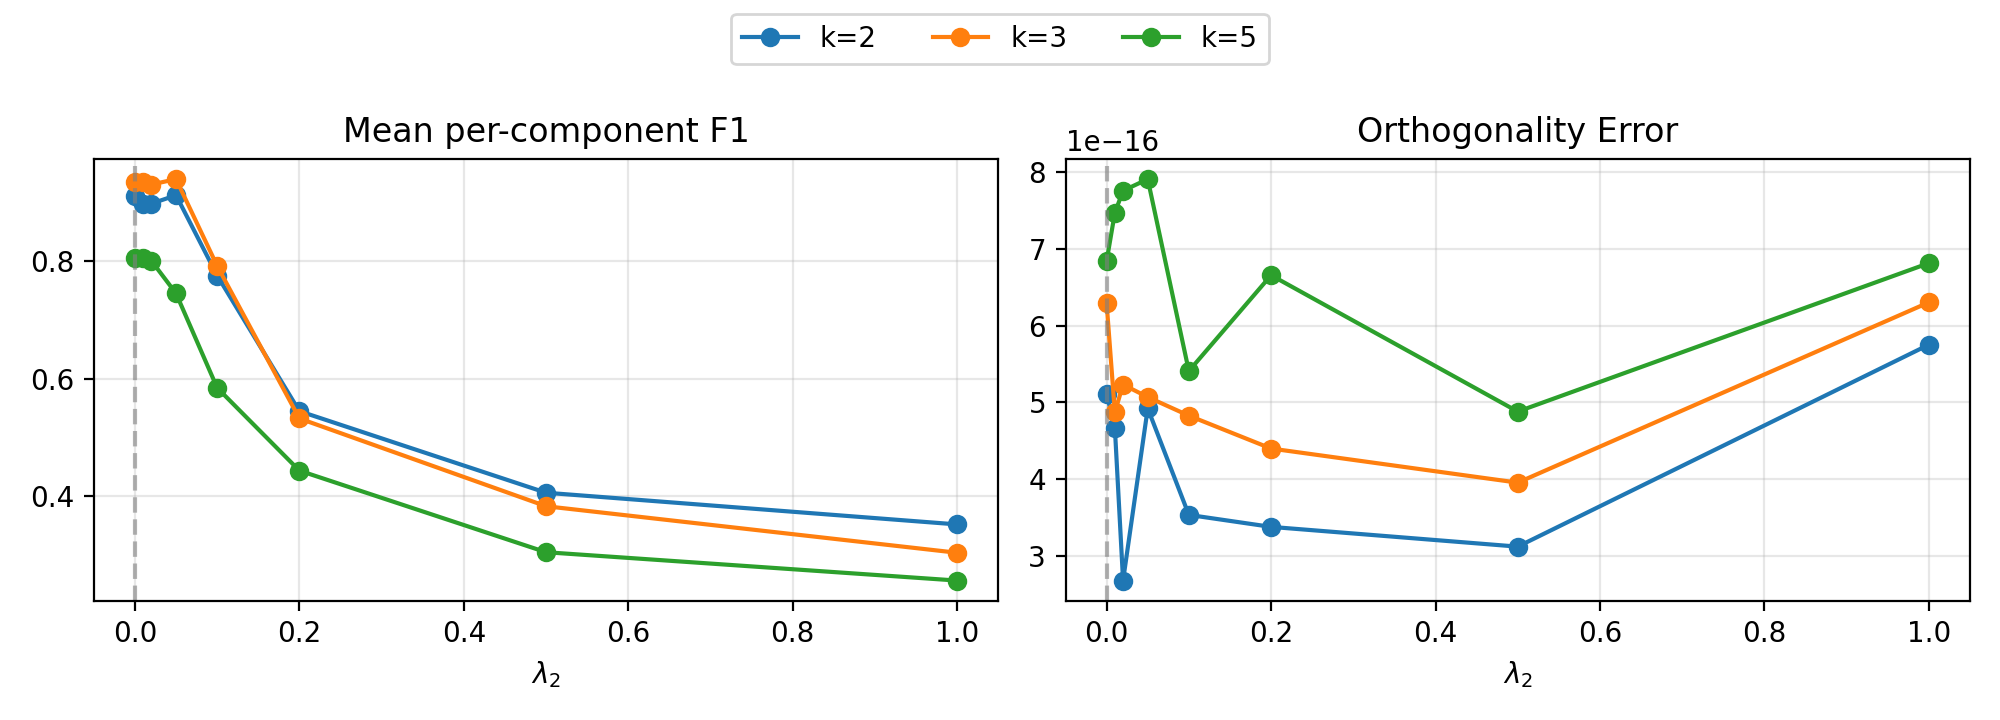
\includegraphics[width=\linewidth]{phase2/multicomponent/multicomp_fragmented_lambda2_sweep.png}
\caption{Multi-component sweep on SBM graphs with fragmented supports. Recovery declines more sharply as $\lambda_2$ increases, while orthogonality remains controlled across $r \in \{2,3,5\}$.}
\label{fig:multicomp-fragmented}
\end{figure}

\begin{figure}[t]
\centering
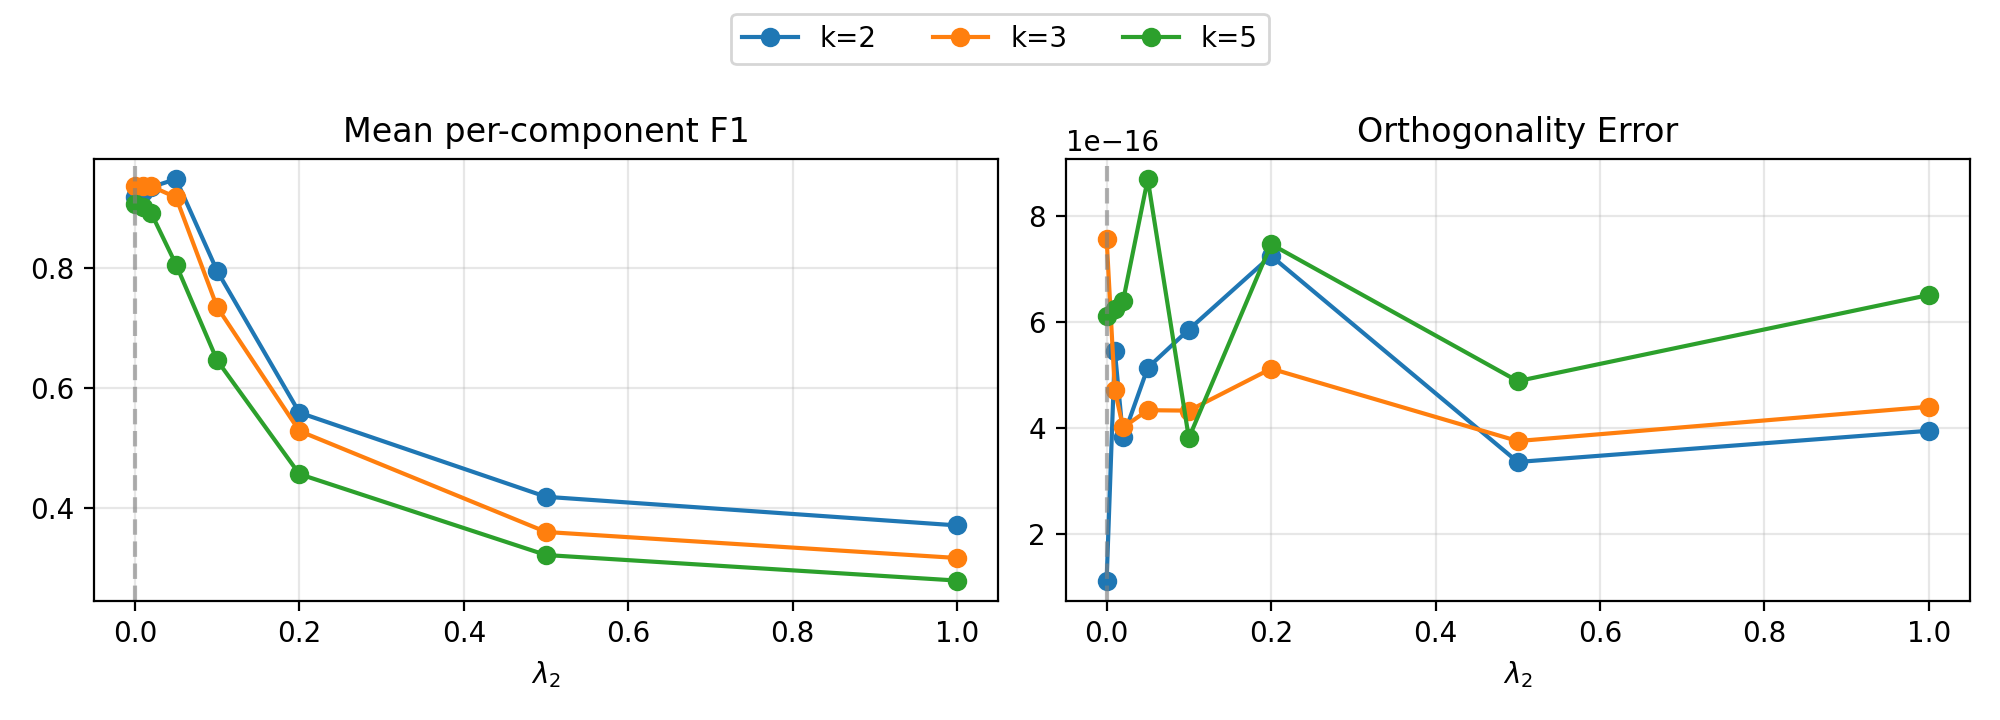
\includegraphics[width=\linewidth]{phase2/multicomponent/multicomp_cross_community_lambda2_sweep.png}
\caption{Multi-component sweep on SBM graphs with cross-community supports. Strong regularization amplifies mismatch, yielding lower recovery at higher $\lambda_2$ despite stable orthogonality.}
\label{fig:multicomp-cross}
\end{figure}

\begin{figure}[t]
\centering
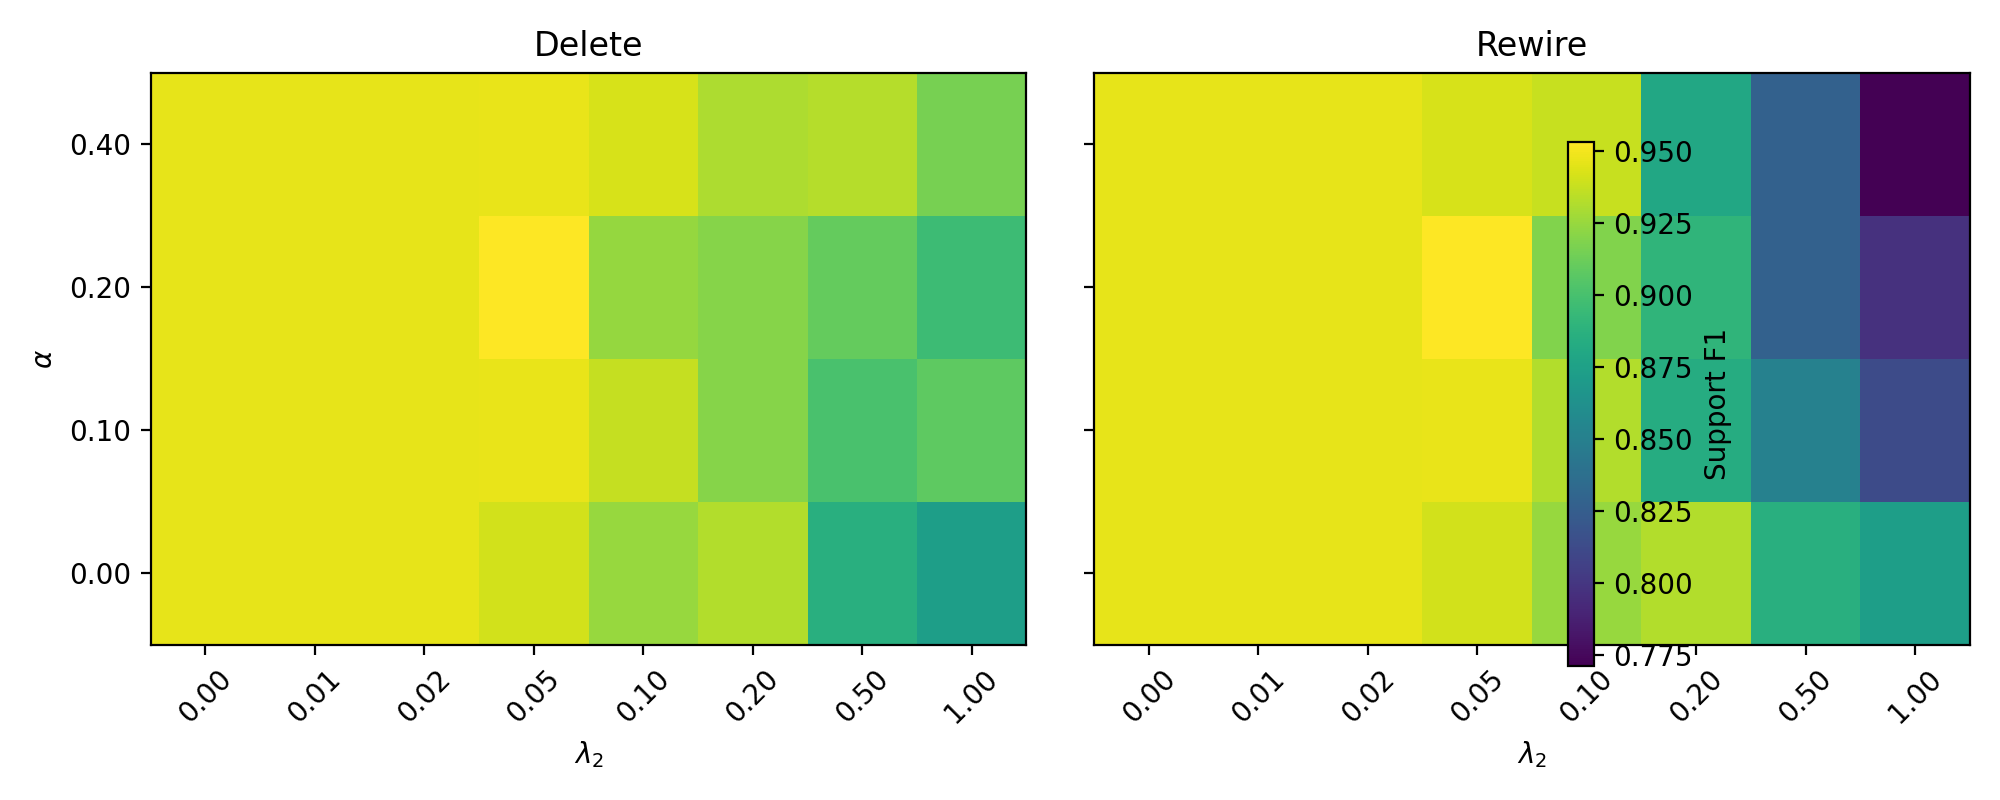
\includegraphics[width=\linewidth]{phase2/compare/phase2_chain_alpha_lambda2_phase_diagram.png}
\caption{Phase diagram on chain graphs. Support F1 as a function of $(\lambda_2,\alpha)$ for deletion (left) and rewiring (right). Sensitivity grows as both $\lambda_2$ and $\alpha$ increase, delimiting a robust low-$\lambda_2$ region.}
\label{fig:phase2-alpha}
\end{figure}

\begin{figure}[t]
\centering
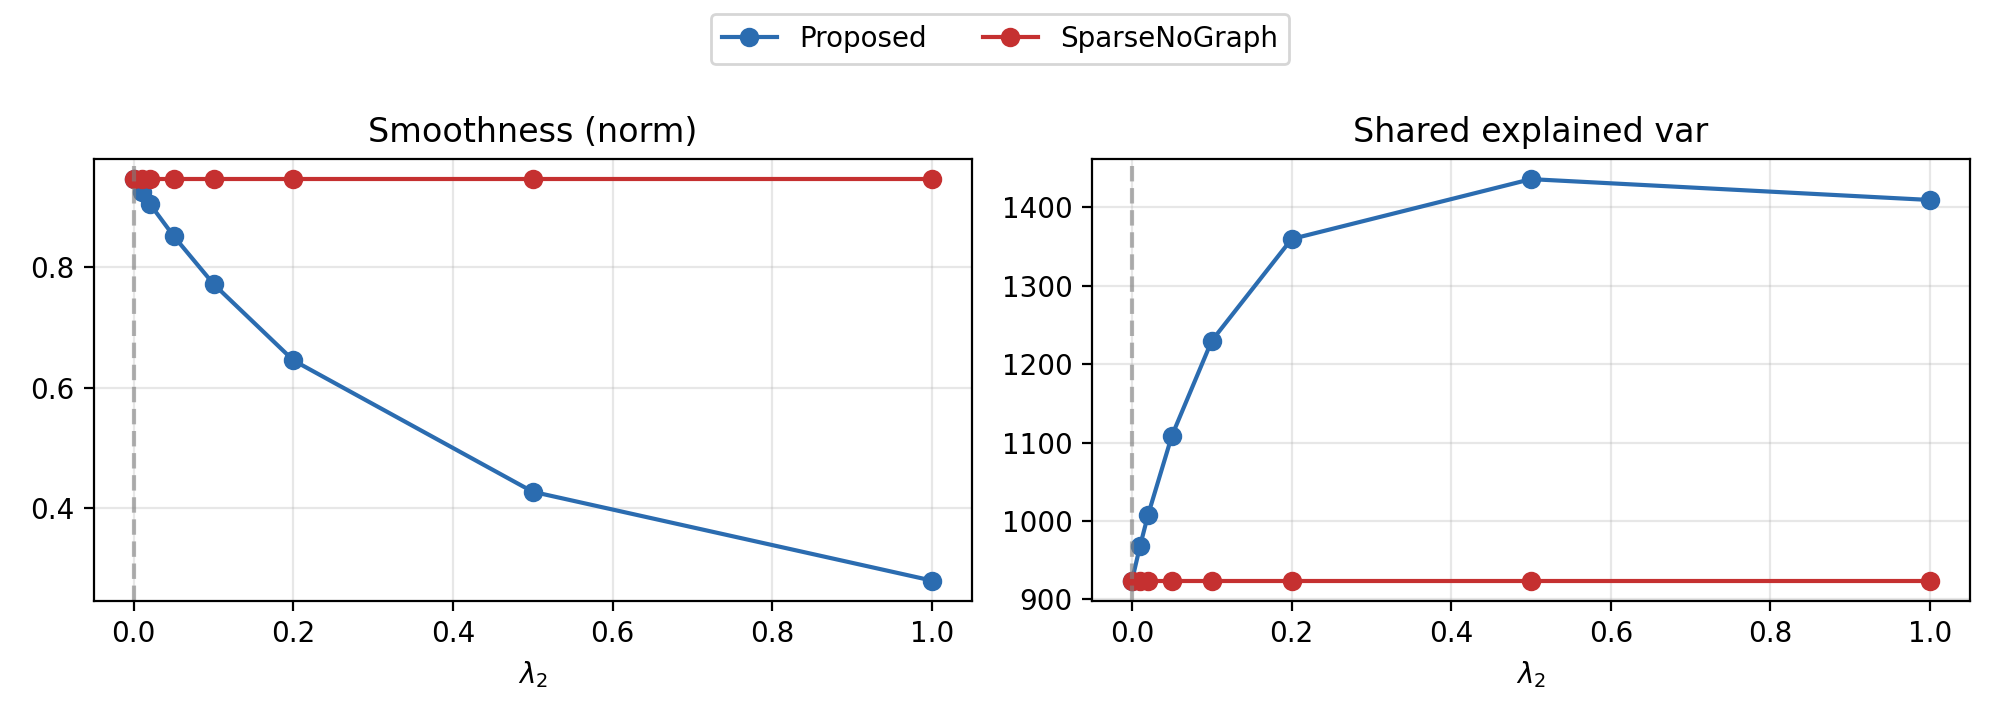
\includegraphics[width=\linewidth]{phase2/realdata/realdata_lambda2_sweep.png}
\caption{Real-data $\lambda_2$ sweep on TCGA-BRCA with STRING graph. Increasing $\lambda_2$ produces progressively smoother solutions, while explained variance improves up to a moderate regime and then plateaus with slight decline at higher $\lambda_2$. This pattern is consistent with the regime behavior observed in synthetic experiments, where moderate regularization yields favorable variance--smoothness tradeoffs and stronger regularization leads to diminishing returns.}
\label{fig:realdata}
\end{figure}

\begin{figure}[t]
\centering
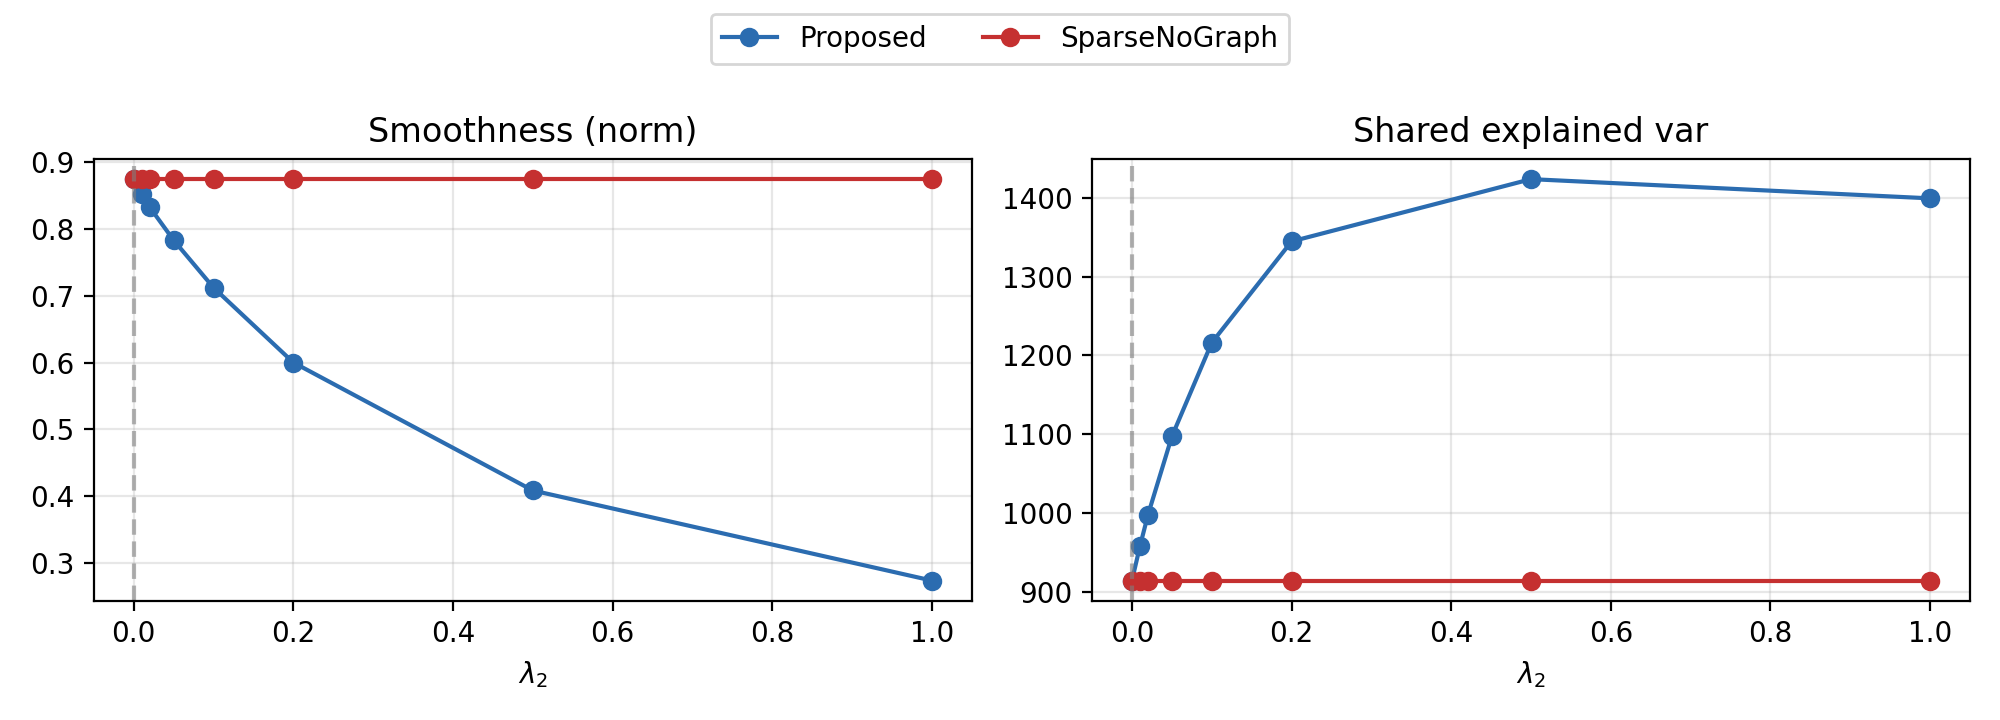
\includegraphics[width=\linewidth]{phase2/realdata/realdata_subsample_lambda2_sweep.png}
\caption{Real-data robustness sweep on TCGA-BRCA under random subsampling. The variance--smoothness tradeoff remains consistent across subsamples, with diminishing variance gains at higher $\lambda_2$.}
\label{fig:realdata-robust}
\end{figure}

\section{Discussion}
\label{sec:discussion}

Our experiments support a regime-based view of graph regularization under misspecification. The effect of the graph prior depends jointly on regularization strength and graph topology. When $\lambda_2$ is small, the prior has limited influence and performance is similar across clean and corrupted graphs. As $\lambda_2$ increases, the prior becomes more influential, and misspecification effects depend on how fragile the underlying topology is.

For chain graphs, misspecification induces clear degradation at moderate-to-high $\lambda_2$, with rewiring more harmful than edge deletion. This indicates that under strong graph regularization, incorrect structure can be more damaging than missing structure. For grid graphs, by contrast, performance remains largely invariant under the same corruption level, suggesting that redundant topology mitigates misspecification effects. In this setting, small performance differences may fluctuate in sign, which we interpret as evidence that the effect is weak and unstable in direction rather than a genuine benefit from misspecification.

A mechanism-level view ties these observations together. The Laplacian term acts as a graph prior whose influence scales with $\lambda_2$: when $\lambda_2$ is small, the data term dominates and the optimizer is insensitive to moderate prior errors; when $\lambda_2$ is large, the prior dominates and any mismatch in graph structure can distort the recovered components.

Topology governs how damaging that distortion becomes. Chains are fragile because smoothness is tied to precise local adjacency, so rewiring directly disrupts the low-frequency directions the prior is meant to promote. Grids are redundant: many neighboring paths induce similar smooth directions, which flattens the optimization landscape and makes performance relatively invariant even when edges are perturbed.

A notable pattern is that rewiring can produce smoother solutions under the corrupted prior without improving alignment with the true graph. This illusory smoothness highlights a critical distinction between smoothness under the imposed prior and structural fidelity measured against the true graph.

\paragraph{Limitations.}
The study remains narrow: we use two synthetic graph families and a single real dataset, and the corruption-strength sweep is reported only for chain graphs. Chain and grid represent two canonical extremes---locally fragile versus redundantly connected---allowing controlled isolation of topology effects. The real-data experiment is intended as a sanity check rather than a comprehensive benchmark, and a formal analysis of regime boundaries is an interesting direction for future work. Broader topology families, multiple real datasets, and systematic corruption sweeps for additional graphs remain important directions for future work. Our claims are therefore intentionally modest: graph regularization is not uniformly beneficial, and its reliability depends on both the strength of regularization and the structural robustness of the imposed graph structure.

\section{Conclusion}
\label{sec:conclusion}

We study graph-smooth sparse orthogonal PCA under controlled graph misspecification and show that its behavior is regime-dependent. At low regularization strength, performance is similar across clean and corrupted graphs, indicating that weak graph priors are comparatively robust. At higher regularization strengths, misspecification effects become topology-dependent: chain graphs exhibit clear degradation, especially under rewiring, whereas grid graphs remain largely invariant under the same perturbations.

These results support a simple but important conclusion: the usefulness of graph regularization is inherently regime- and topology-dependent. Strong graph priors can amplify structural errors in fragile graphs, while redundant topologies mitigate those effects. This suggests that graph regularization should be interpreted not as a universally helpful inductive bias, but as a topology- and regime-sensitive mechanism whose reliability depends on the quality and robustness of the imposed graph structure. Practically, this suggests that graph regularization should be used conservatively unless the graph structure is known to be reliable or topologically redundant.

\fussy
\bibliographystyle{plain}
\bibliography{references}

\end{document}
